\let\negmpace\undefined
\let\negthickspace\undefined
\documentclass[journal]{IEEEtran}
\usepackage[a5paper, margin=10mm, onecolumn]{geometry}
%\usepackage{lmodern} % Ensure lmodern is loaded for pdflatex
\setlength{\headheight}{1cm} % Set the height of the header box
\setlength{\headsep}{0mm}     % Set the distance between the header box and the top of the text
\usepackage{xparse}
\usepackage{gvv-book}
\usepackage{gvv}
\usepackage{cite}
\usepackage{amsmath,amssymb,amsfonts,amsthm}
\usepackage{algorithmic}
\usepackage{graphicx}
\usepackage{textcomp}
\usepackage{xcolor}
\usepackage{txfonts}
\usepackage{listings}
\usepackage{enumitem}
\usepackage{mathtools}
\usepackage{gensymb}
\usepackage{comment}
\usepackage[breaklinks=true]{hyperref}
\usepackage{tkz-euclide} 
\usepackage{listings}
% \usepackage{gvv}                                        
\def\inputGnumericTable{}                                 
\usepackage[latin1]{inputenc}                                
\usepackage{color}                                            
\usepackage{array}                                            
\usepackage{longtable}                                       
\usepackage{calc}                                             
\usepackage{multirow}                                         
\usepackage{hhline}                                           
\usepackage{ifthen}                                           
\usepackage{lscape}
\renewcommand{\thefigure}{\theenumi}
\renewcommand{\thetable}{\theenumi}
\setlength{\intextsep}{10pt} % Space between text and floats
\numberwithin{equation}{enumi}
\numberwithin{figure}{enumi}
\renewcommand{\thetable}{\theenumi}
\begin{document}
\bibliographystyle{IEEEtran}
\title{Question-7-7.2-8}
\author{EE24BTECH11033 - KOLLURU SURAJ}
% \maketitle
% \newpage
% \bigskip
{\let\newpage\relax\maketitle}
\textbf{Question}:\\
The centre of circle is $\brak{2a,a-7}$. Find the values of a if the circle passes through the point $\vec{A}\brak{11,-9}$and has diameter $10\sqrt{2}$ units 
\\
\solution \\
\begin{table}[!ht]
  \centering
  \begin{tabular}{ |c| c|}
    \hline
    \textbf{point}  &  \textbf{Coordinates}\\
    \hline
    $\vec{A}$ & $\brak{-4,6}$ \\
    \hline
    $\vec{B}$ & $\brak{-4,-6}$\\
    \hline
    $\vec{C}$ & $\brak{-4,2}$\\
    \hline
\end{tabular}    


  \caption{variables used}
\end{table}\\
The radius of circle is $\frac{diameter}{2}$
\begin{align}
    \implies radius=5\sqrt{2}\\
    \norm{\vec{A}-\vec{C}} &= 5\sqrt{2}\\
    \vec{A}-\vec{C} &= \myvec{11-2a \\ -2-a}\\
    \brak{11-2a}^2 +\brak{2+a}^2 &= 50\\
    a^2-8a+15 &= 0\\
    \brak{a-3}\brak{a-5}&=0\\
	\therefore  a =3 \text{ or } a = 5
\end{align}
\begin{figure}[!ht]
    \centering
    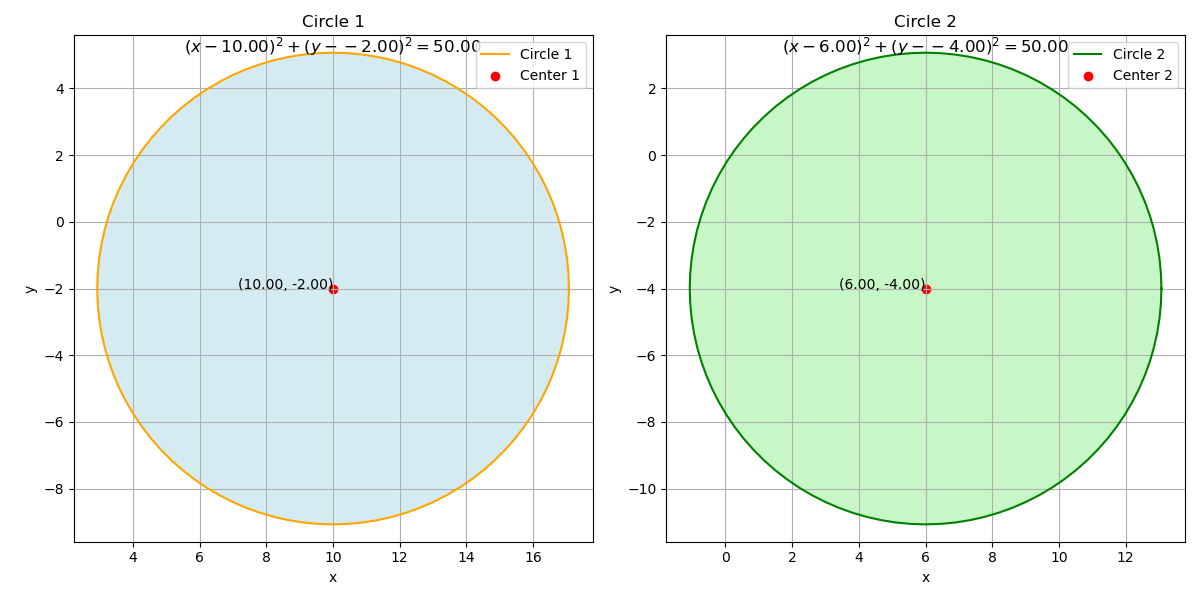
\includegraphics[width=\linewidth]{figs/Figure_1.png}
    \caption{}
\end{figure}

\end{document}
